\documentclass{report}
\usepackage[english]{babel}
\usepackage[utf8]{inputenc}
\usepackage[T1]{fontenc}
\usepackage{listings}
\usepackage{titlesec}
\usepackage{color}
\usepackage{graphicx}

\titleformat{\chapter}[display]
            {\normalfont\bfseries}{}{0pt}{\Huge}

\lstset{ escapeinside={(*}{*)} }

\title{Méthodes et Outils pour la Conception Avancée}
\author{Castel Antonin, Reboul Paul, Vandendorpe Thomas}
\begin{document}
\maketitle{}
\tableofcontents

\chapter{Introduction}

Ce dossier rassemble les travaux effectués lors du cours de ``Méthodes et Outils pour la Conception Avancée''. L'objectif ici, est de montrer les bonnes pratiques à avoir lors de la conception d'un programme. Nous illustrerons ces bonnes pratiques à partir de l'exemple d'un programme de puissance 4 (en langage C), initialement codé de façon peu rigoureuse, que nous tenterons d'améliorer tout au long de ce dossier. Par améliorer, on entend  la maintenabilité, la réutilisabilité et la documentation du code, la qualité et la couverture des tests, la détection de défauts et d'erreurs, l'analyse et l'amélioration des performances, ainsi que l'analyse de la vulnérabilité à certaines attaques. Nous expliquerons les différentes méthodes et outils permettant ces améliorations...

\chapter{Modularité, maintenabilité, réutilisabilité}
\section{Structuration}
L'élément le plus important pour gagner du temps dans notre travail, est l'organisation. La première chose que l'on commence à faire, est de structurer le code en parties pour s'y retrouver le mieux possible. Cela implique de rassembler les fonctions par thèmes dans différents fichiers. Lors de la séparation en plusieurs fichiers, les variables globales initiales sont devenues obsolètes, laissant place à un type struct plus facile d'utilisation entre les fichiers. L'application est désormais décomposée en plusieurs modules ce qui permet de faire des tests unitaires indépendamment des autres, mais aussi de trouver et corriger des erreurs plus facilement lors de la compilation. Dans le cas de notre puissance 4, nous avons séparé l'application en 5 fichiers :
\begin{itemize}
\item appli.c : contient la fonction main
\item board.c/board.h : les fonctions manipulant la structure board (le plateau de puissance 4)
\item action.c/action.h : les actions (les règles) du jeu
\item ia.c/ia.h : les IAs
\item score.c/score.h : les informations de scores
\end{itemize} 
Pour que l'environnement de travail soit propre et accessible, on regroupe les fichiers sources dans un même dossier, de même pour les includes, les tests et documents de sorte à faciliter la chercher des fichiers.


\section{Documentation}
Pour que le code d'une application soit compris par un large public, sans devoir expliquer chaque fonction du code en détail, on emploie une méthode de normage global. Comme par exemple, le renommage des variables et des fonctions selon leur usage, ce qui permet une compréhension plus aisée du code. D'autre part, Doxygen permet de faire une documentation succincte, il suffit d'écrire un commentaire pour chaque fonction, décrivant son utilisation et fonctionnement. Doxygen permet d'avoir une documentation élémentaire et simple à mettre à jour.
Exemple d'utilisation de Doxygen:
\begin{scriptsize}
\begin{lstlisting}
/**
* \file  board.c
* \brief Gestion de la grille de jeu ainsi que des scores 
*/

/**
 * \brief      Cree une table de jeu
 * \details    initialisation de la grille de jeu ainsi que des scores
 * \param      width         largeur de la grille
 * \param      heigh         longueur de la grille
 * \param      highscores    table des highscores
 * \return     une grille de jeu selon les parametres donnes
 */
Board board_new(int width,int height,int highScores){
  Board b;
  int i,j;
  b.tab = (char **)malloc(height*sizeof(char *));
  b.width = width;
  b.height = height;
  b.highScores = highScores;
  for(i=0; i<height; i++)
    {
      b.tab[i] = (char*)malloc(width*sizeof(char));
      for(j=0; j<width; j++)
  {
    b.tab[i][j]= VIDE;
  }
    }
  b.last = malloc(width*height*sizeof(char));
  b.n_last = 0;
  b.undoRedoIndex = 0;
  return b;
}

\end{lstlisting}
\end{scriptsize}
\begin{center}
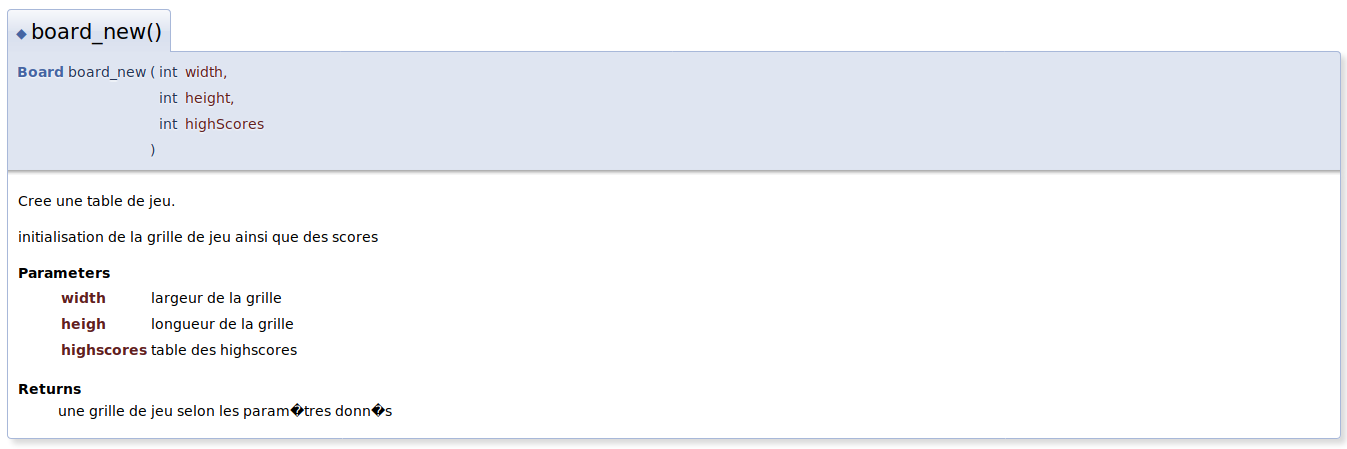
\includegraphics[width=13cm]{board.png}
\end{center}

\chapter{Qualité des tests}
On ne peut pas parler de qualité du logiciel sans parler des tests. Bien que ne prouvant pas l'absence de bug dans un code, les tests exécutés sur un programme sont de bons indicateurs sur sa qualité. Il est nécessaire de ``penser tests'' tôt dans la création d'un logiciel, car les tests sont écrits au fur et à mesure de la conception et sont destinés à être exécutés plusieurs fois, ceci afin de vérifier que les modifications et ajouts dans le code permettent toujours de valider les tests précédents. Et ceci est d'autant plus vrai lors d'un projet en équipe où les modifications des uns peuvent affecter les modifications des autres. Nous allons dans cette partie présenter deux méthodes permettant d'assurer une certaine rigueur dans les tests : l'une au sujet des tests unitaires et la seconde concernant l'analyse de couverture.
\section{Les tests unitaires}
Les tests unitaires sont des tests s'appliquant à une partie d'un programme et permettant de vérifier le programme par bloc. Un bloc de programme est en fait une fonction, et l'idée est d'écrire un test qui appelle une certaine fonction avec certains paramètres (judicieusement choisis si possible, c'est-à-dire couvrant le plus de branches possibles) et de vérifier que le résultat renvoyé par la fonction est bien le résultat attendu. Il est possible d'écrire ces tests en suivant un processus de développement dirigé par les tests, qui consiste à écrire les tests avant d'écrire la fonction correspondante. Mais on peut également les écrire si on dispose déjà de la fonction à tester en utilisant sa spécification (qui devrait être facilement accessible si le code a été documenté avec un outil adéquat), ce qui arrive si l'on est amené à retoucher un code existant.

TODO : Nécessiter de prendre en compte/modifier des fonctions pour permettre le test unitaire (valeur retour, etc.) + découpage code en fonction.
\paragraph{Exemple}
Illustrons ce principe de tests unitaires à l'aide d'un exemple tiré d'un programme de puissance 4 (en langage C). Nous souhaitons écrire un test pour la fonction suivante :

\begin{scriptsize}
\begin{lstlisting}

int checkfull(Board board);

/*
*Verifie si une grille(Board) est pleine
*
*Parameters
*   board: une table de jeu
*
*Returns
*   0 si la grille est pleine, 1 sinon
*/


\end{lstlisting}
\end{scriptsize}

Il existe de nombreux frameworks permettant l'automatisation des tests unitaires, dans cet exemple, on utilise CuTest. Il peut être intéressant de remarquer (en gras) l'assignation des "variable actual" (valeur renvoyée par la fonction testée), de "expected" (valeur attendue) et leur comparaison (qui fonctionne un peu comme une assertion).
\begin{scriptsize}
\begin{lstlisting}

void Test_checkfull(CuTest *tc){
  int i,j,expected,actual;
  Board b=boardVide(15,22);
  for(i=0;i<b.height;i++){
    for(j=1;j<=b.width;j++){
      (*\bfseries actual = checkfull(b);*)
      (*\bfseries expected = 1;*)
      (*\bfseries CuAssertIntEquals(tc, expected, actual);*)
      board_put(&b,j);
    }
  }
   (*\bfseries actual = checkfull(b); *)
   (*\bfseries expected = 0; *)
   (*\bfseries CuAssertIntEquals(tc, expected, actual); *)
}

\end{lstlisting}
\end{scriptsize}

Les tests écrits de cette façon pourront ensuite tous être exécutés en même temps et des informations sur les échecs des tests seront disponibles :

\begin{scriptsize}
\begin{lstlisting}

.......F.........

There was 1 failure:
1) Test_checkfull: src/CuTestTest.c:221: expected <0> but was <1>

!!!FAILURES!!!
Runs: 17 Passes: 16 Fails: 1

\end{lstlisting}
\begin{lstlisting}

.................

OK (17 tests)
\end{lstlisting}
\end{scriptsize}

Comme les tests sont ensuite faciles à relancer, il est important de les réexécuter à chaque changement important dans le code afin d'éviter la régression.

\section{Couverture}
La couverture est un indicateur permettant de savoir quelles parties du code ont été couvertes par les tests. Utiliser la couverture seule n'est pas forcément intéressant, puisqu'elle n'indique pas si les tests ont été validés ou non. En revanche, en combinaison des tests unitaires vu précédemment, on a un indicateur de la qualité des tests très puissant puisqu'on a l'information du pourcentage du code testé et du nombre de tests validés.
\paragraph{Exemple}
Nous avons utilisé l'outil gcov afin d'observer la couverture de notre puissance 4. Comme ce dernier ne donne qu'un résultat textuel de la couverture, nous avons complété son utlisation avec l'outil lcov, qui utilise ce que gcov a produit mais rajoute une interface html afin que la couverture soit plus facile à lire. On peut ainsi observer le pourcentage de lignes/fonctions visitées par les tests :

\begin{center}
  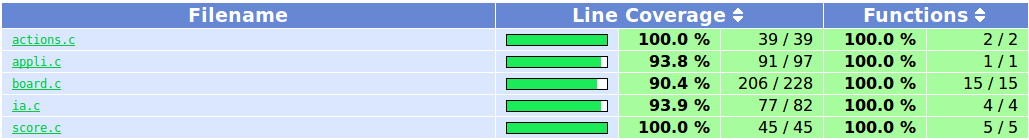
\includegraphics[width=13cm]{couverture1.png}
\end{center}

En plus des pourcentages de couverture, on peut également directement voir sur le code ce qui a été couvert (en bleu) et ce qui ne l'a pas été (en rouge). Cela est pratique lorsqu'on écrit des tests en essayant de passer par le plus de branches possibles (conditions, boucles, ...) du programme.

\begin{center}
  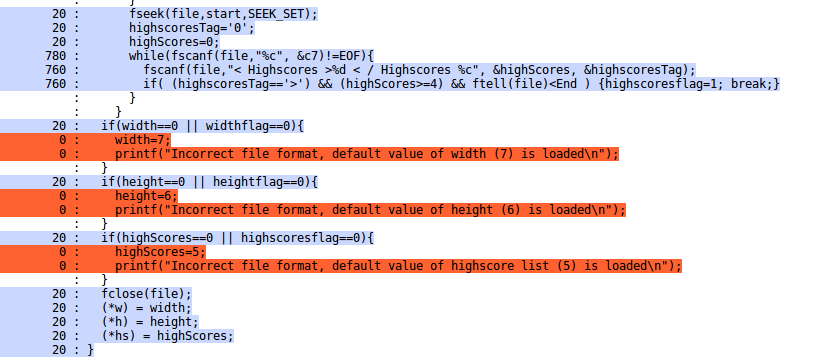
\includegraphics[width=13cm]{couverture2.png}
\end{center}

\chapter{Détection de défauts et erreurs}
Bien que les tests permettent de trouver les bugs les plus gros dans un programme, on ne peut souvent pas tester tous les états possibles, et il peut rester des bugs arrivant dans certains cas particuliers, ou bien des défauts non directement visibles. On peut alors se tourner vers des outils spécialisés dans la détection d'erreurs. Nous allons ainsi voir deux types d'outils : un débogueur et un outil d'exécution symbolique.
\section{Débogueur}
Un débogueur permet de contrôler l'exécution d'un programme et ajoute des informations supplémentaires à ce dernier. On peut ainsi détecter des erreurs comme des accès mémoire non autorisés, ou bien même des fuites mémoire.
\paragraph{Exemple}
Le puissance 4 que nous sommes en train de modifier déclenche des erreurs de segmentation dans certains cas. Nous allons donc utiliser un outil de débogage simple d'utilisation : valgrind. Il suffit d'exécuter notre programme avec valgrind pour que ce dernier nous détaille la provenance de l'erreur :

\begin{scriptsize}
  \begin{lstlisting}

==2528== Invalid read of size 8
==2528==    at 0x408ACF: checkEmpty1 (ia.c:34)
==2528==    by 0x409368: Medium (ia.c:93)
==2528==    by 0x405C66: play_ia (actions.c:20)
==2528==    by 0x402631: main (appli.c:146)
    
  \end{lstlisting}
\end{scriptsize}

On a ainsi accès à la ligne, à la suite d'appel des fonctions et à la taille de l'accès mémoire ayant déclenché l'erreur, il ne reste qu'à la corriger en ajoutant des conditions (voire des assertions) anticipant les accès non autorisés. En vert les corrections ajoutées :

\begin{scriptsize}
  \begin{lstlisting}
int checkEmpty1(Board b,int num,int numOfrow)
{
  (*\color{green} assert(num>=0 \&\& num<b.width);*)
  (*\color{green} assert(numOfrow>=0 \&\& numOfrow<b.height);*)
  if(numOfrow==(b.height-1) && b.tab[numOfrow][num]==VIDE){
    return 1;
  }
  else if((*\color{green} numOfrow+1<b.height \&\& *) b.tab[numOfrow+1][num]!=VIDE && b.tab[numOfrow][num]==VIDE){
    return 1;
  }
  return 0;
}
  \end{lstlisting}
\end{scriptsize}

A noter que Valgrind nous donne également des informations sur les fuites mémoire en nous informant sur le nombre de blocs alloués/libérés.

\begin{scriptsize}
  \begin{lstlisting}
==2869== HEAP SUMMARY:
==2869==     in use at exit: 42 bytes in 1 blocks
==2869==   total heap usage: (*\bfseries 26 allocs, 25 frees *), 100,764 bytes allocated
==2869== 
==2869== 42 bytes in 1 blocks are definitely lost in loss record 1 of 1
==2869==    at 0x4C2DB8F: malloc (in /usr/lib/valgrind/vgpreload_memcheck-amd64-linux.so)
==2869==    by 0x406695: board_new (board.c:35)
==2869==    by 0x401609: main (appli.c:21)
  \end{lstlisting}
\end{scriptsize}

\section{Exécution symbolique}
Cette méthode pour trouver des bugs dans un programme consiste à explorer tous les chemins d'exécution possibles de ce programme. Bien que cette méthode donne de bons résultats, elle a l'inconvéniant de ne s'appliquer qu'à de petits codes (ou petites portions de codes) ceci étant dû au nombre de chemins explorés selon la taille du code. 

\paragraph{Exemple}
Nous avons utilisé Klee sur notre programme. Klee nécessite d'instrumenter son code afin de désigner quelles variables peuvent voir leur valeur changer. Dans notre cas, il s'agit des entrées de l'utilisateur.

En lançant Klee et en attendant quelques minutes, on a pu débusquer une erreur d'accès mémoire via le message suivant :
\begin{scriptsize}
  \begin{lstlisting}
KLEE: ERROR: appli.c:641: memory error: out of bound pointer
  \end{lstlisting}
\end{scriptsize}

Même une fois l'erreur trouvée, Klee continue à tourner et cherche d'autres problèmes.
\chapter{Analyse de performance}
Au-delà de l'aspect programmation, qui se doit d'être affiné le plus possible afin que le programme s’exécute dans un temps minimal, nous avons optimisé le programme afin de minimiser les temps d'accès aux caches du processeur.
En effet, une erreur de prédiction de saut ou une donnée non présente dans un cache lors de l’accès fait perdre un temps considérable dans l'exécution du programme. Il faut dans un cas, détecter l'erreur de branchement et la corriger, et dans l'autre cas, aller chercher la donnée dans la mémoire.
Pour optimiser cet aspect, on peut citer deux bonnes pratiques simples : 
\newline
- Remplacer les séries de "if" par des "switch", car la table de branchement de ce dernier minimise le pourcentage de "branch miss". 
\newline
- Changer les ordres de parcours des tableaux dans la mesure du possible afin de minimiser cette fois le pourcentage de "cache miss".
\newline
Sur un petit programme, ces optimisations peuvent ne pas être visibles et semblées anecdotiques mais sur un projet de plus grande envergure, optimiser cet aspect est essentiel.

\paragraph{Exemple}
Nous avons travaillé avec l'option "Cachegrind" de Valgrind pour détecter et dénombrer le taux de miss.
On peut voir sur le tableau suivant un certain nombre d'informations qui représentent le pourcentage de miss des différents caches, ainsi que le nombre concret de miss. 
Nous pouvons aussi voir le pourcentage de "branch miss" dans les dernières lignes. 
Ce tableau est extrait d'une exécution de Cachegrind sur la version de base du projet, avant toute modification (hormis celles qui permettent simplement au programme de compiler).
Ce tableau se comprend comme ceci :
\newline
I fait référence au cache instruction, I1 au cache le plus rapide d'accès et LL (pour "last level") aux caches plus éloignés.
\newline
D fait référence au cache de données (Data) et fonctionne sur le même principe.
Les branchements quant à eux sont simplement énoncés à la fin de l'analyse.

\begin{scriptsize}
\begin{lstlisting}
==4891== 
==4891== I   refs:      4,320,762
==4891== I1  misses:       14,181
==4891== LLi misses:        1,990
==4891== I1  miss rate:      0.33%
==4891== LLi miss rate:      0.05%
==4891== 
==4891== D   refs:      1,758,266  (1,140,077 rd   + 618,189 wr)
==4891== D1  misses:        3,357  (    2,709 rd   +     648 wr)
==4891== LLd misses:        2,668  (    2,086 rd   +     582 wr)
==4891== D1  miss rate:       0.2% (      0.2%     +     0.1%  )
==4891== LLd miss rate:       0.2% (      0.2%     +     0.1%  )
==4891== 
==4891== LL refs:          17,538  (   16,890 rd   +     648 wr)
==4891== LL misses:         4,658  (    4,076 rd   +     582 wr)
==4891== LL miss rate:        0.1% (      0.1%     +     0.1%  )
==4891== 
==4891== Branches:        804,931  (  754,035 cond +  50,896 ind)
==4891== Mispredicts:      20,138  (   19,816 cond +     322 ind)
==4891== Mispred rate:        2.5% (      2.6%     +     0.6%   )
\end{lstlisting}
\begin{center}
\textbf{\textit{Figure 1 : Execution de Cachegrind sur le programme de base.}}
\end{center}
\end{scriptsize}

Après les modifications de notre programme, nous avons obtenu les valeurs suivantes, qui s’interprètent exactement de la même façon.
\begin{scriptsize}
\begin{lstlisting}
==5578== 
==5578== I   refs:      5,222,873
==5578== I1  misses:        2,457
==5578== LLi misses:        1,762
==5578== I1  miss rate:      0.05%
==5578== LLi miss rate:      0.03%
==5578== 
==5578== D   refs:      2,167,133  (1,304,576 rd   + 862,557 wr)
==5578== D1  misses:        6,828  (    4,225 rd   +   2,603 wr)
==5578== LLd misses:        4,814  (    2,422 rd   +   2,392 wr)
==5578== D1  miss rate:       0.3% (      0.3%     +     0.3%  )
==5578== LLd miss rate:       0.2% (      0.2%     +     0.3%  )
==5578== 
==5578== LL refs:           9,285  (    6,682 rd   +   2,603 wr)
==5578== LL misses:         6,576  (    4,184 rd   +   2,392 wr)
==5578== LL miss rate:        0.1% (      0.1%     +     0.3%  )
==5578== 
==5578== Branches:      1,073,634  (1,001,931 cond +  71,703 ind)
==5578== Mispredicts:      24,986  (   22,529 cond +   2,447 ind)
==5578== Mispred rate:        2.3% (      2.5%     +     3.4%   )
\end{lstlisting}
\begin{center}
\textbf{\textit{Figure 2 : Exécution de Cachegrind sur le programme. modifié}}
\end{center}

Comme on peut le voir, le nombre de "cache miss" à grandement diminué vu que nous sommes passés de 0.33\% à 0.05\%. 
\newline
Il serait probablement possible d'améliorer encore ce score mais cela demanderait beaucoup de temps car cela nécessiterait de reprendre un grand pourcentage du code, ce qui ne vaut pas forcément le coup étant donné que 0.05\% de miss est un score correct.
\newline
Pour ce qui est des prédictions de branchements, elles ont très peu diminuées car les améliorations que nous avons faites sont peu nombreuses, le programme ne se prête pas vraiment à ce genre d'optimisation.
\newline
Il est à noter qu'il est normal d'avoir quelques "branch miss" sur un programme de cette taille.
\end{scriptsize}

\end{document}